
\chapter{Radiogoniometre}

Pour réaliser notre projet nous avons été obligé d'adapter notre capteur le radiogoniomètre Montréal 3v2 a nos besoin.

\section{Down converter}


\begin{wrapfigure}{r}{0.4\textwidth}
  
  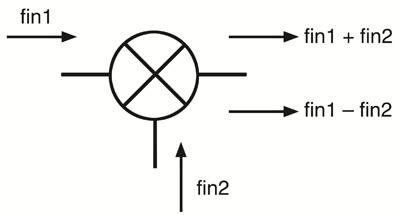
\includegraphics[width=0.4\textwidth]{mixer}
  \caption{schéma de fonctionnement d'un mixer}
\end{wrapfigure}


Le radiogoniomètre Montréal 3v2 fonctionne à une fréquence de 500Mhz. Il est donc impossible de l’utilisé entre 2.4Ghz et 2.5 GHz, bande de fréquence qu’utilise les drones que nous souhaitons utiliser. Nous avons donc cherché un moyen d’adapter ce radiogoniomètre aux fréquences souhaitées.


Nous avons trouvé une solution applicable à notre système.

D’abord nous avons utilisé un down-converter. Ce composant reçoit deux entrées, le signal dont on veut changer la fréquence(RF) et un signal de fréquence Df(LO). Le down-converter diminue la fréquence du premier signal de celle du second. La sortie(IF) correspond au signal modifié. Son principe de fonctionnement est illustré à la figure \ref{fig:mix}.



\begin{figure}[h]
  \centering
  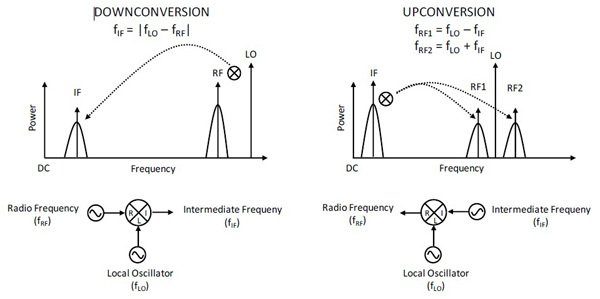
\includegraphics[width=\textwidth]{fonc_mixer}
  \caption{principe du fonctionnement d'un mixer}
  \label{fig:mix}
\end{figure}

Dans ce cadre on utilise le down-converter pour diminuer la fréquence.
La fréquence du signal Df est donnée par un VCO, le VCO reçoit en entrée une tension et donne en sortie une sinusoïdal de fréquence dépendante de la tension d’entrée. Le VCO étant très sensible, il est nécessaire de stabilisé la tension d’entrée et l’alimentation. On utilise donc un régulateur de tension qui amène une entrée stable. Il en a fallu un second pour alimenter le VCO, toujours dans le but d’obtenir une fréquence stable ne variant pas pendant le processus, 

Il est en effet indispensable que cette fréquence reste fixe pour ne pas parasité l’effet doppler, la combinaison des deux indiquerait une mauvaise position.
Le régulateur reçoit une tension V, si V est supérieur à la tension Vmax du régulateur, la tension de sortie devient Vmax. 

Après il a fallu gérer du signal d’entrée du down-converter et des problèmes de bruit, on a donc placé un filtre devant le down-converter. Ce filtre est un filtre passe bande qui fonctionne autour de 2.4Ghz-2.5Ghz pour ne garder que ce qui nous intéresse.


\begin{figure}[h]
  \centering
  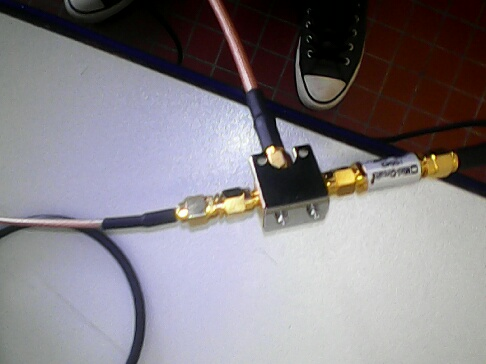
\includegraphics[width=0.5\textwidth]{down_converter}
  \caption{le down-converter et le filtre passe bande}
  \label{fig:down}
\end{figure}

A l’aide de ce montage on peut abaisser la fréquence du signal d’entrée.

%%% Local Variables: 
%%% mode: latex
%%% TeX-master: "../rapport"
%%% End: 
